
%%%%%%%%%%%%%%%%%%%%%%%%%%%%%%%%%%%%%%%%%%%%%%%%%%%%%%%%%%%%%%%%%%%%%%%%%%%%%%%%%%%%%%%
%%%%%%%%%%%%%%%%%%%%%%%%%%%%%%%%%%%%%%%%%%%%%%%%%%%%%%%%%%%%%%%%%%%%%%%%%%%%%%%%%%%%%%%
% 
% This top part of the document is called the 'preamble'.  Modify it with caution!
%
% The real document starts below where it says 'The main document starts here'.

\documentclass[12pt]{article}

\usepackage{amssymb,amsmath,amsthm}
\usepackage[top=1in, bottom=1in, left=1.25in, right=1.25in]{geometry}
\usepackage{fancyhdr}
\usepackage{enumerate}
\usepackage{listings}
\usepackage{graphicx}
\usepackage{float}

\usepackage{mwe}
\usepackage{caption}
\usepackage{subcaption}
% Comment the following line to use TeX's default font of Computer Modern.
\usepackage{times,txfonts}



\makeatletter
\renewcommand*\env@matrix[1][*\c@MaxMatrixCols c]{%
  \hskip -\arraycolsep
  \let\@ifnextchar\new@ifnextchar
  \array{#1}}
\makeatother

\newtheoremstyle{homework}% name of the style to be used
  {18pt}% measure of space to leave above the theorem. E.g.: 3pt
  {12pt}% measure of space to leave below the theorem. E.g.: 3pt
  {}% name of font to use in the body of the theorem
  {}% measure of space to indent
  {\bfseries}% name of head font
  {:}% punctuation between head and body
  {2ex}% space after theorem head; " " = normal interword space
  {}% Manually specify head
\theoremstyle{homework} 

% Set up an Exercise environment and a Solution label.
\newtheorem*{exercisecore}{Exercise \@currentlabel}
\newenvironment{exercise}[1]
{\def\@currentlabel{#1}\exercisecore}
{\endexercisecore}

\newcommand{\localhead}[1]{\par\smallskip\noindent\textbf{#1}\nobreak\\}%
\newcommand\solution{\localhead{Solution:}}

%%%%%%%%%%%%%%%%%%%%%%%%%%%%%%%%%%%%%%%%%%%%%%%%%%%%%%%%%%%%%%%%%%%%%%%%
%
% Stuff for getting the name/document date/title across the header
\makeatletter
\RequirePackage{fancyhdr}
\pagestyle{fancy}
\fancyfoot[C]{\ifnum \value{page} > 1\relax\thepage\fi}
\fancyhead[L]{\ifx\@doclabel\@empty\else\@doclabel\fi}
\fancyhead[C]{\ifx\@docdate\@empty\else\@docdate\fi}
\fancyhead[R]{\ifx\@docauthor\@empty\else\@docauthor\fi}
\headheight 15pt

\def\doclabel#1{\gdef\@doclabel{#1}}
\doclabel{Use {\tt\textbackslash doclabel\{MY LABEL\}}.}
\def\docdate#1{\gdef\@docdate{#1}}
\docdate{Use {\tt\textbackslash docdate\{MY DATE\}}.}
\def\docauthor#1{\gdef\@docauthor{#1}}
\docauthor{Use {\tt\textbackslash docauthor\{MY NAME\}}.}
\makeatother

% Shortcuts for blackboard bold number sets (reals, integers, etc.)
\newcommand{\Reals}{\ensuremath{\mathbb R}}
\newcommand{\Nats}{\ensuremath{\mathbb N}}
\newcommand{\Ints}{\ensuremath{\mathbb Z}}
\newcommand{\Rats}{\ensuremath{\mathbb Q}}
\newcommand{\Cplx}{\ensuremath{\mathbb C}}
%% Some equivalents that some people may prefer.
\let\RR\Reals
\let\NN\Nats
\let\II\Ints
\let\CC\Cplx
%%%%%%%%%%%%%%%%%%%%%%%%%%%%%%%%%%%%%%%%%%%%%%%%%%%%%%%%%%%%%%%%%%%%%%%%%%%%%%%%%%%%%%%
%%%%%%%%%%%%%%%%%%%%%%%%%%%%%%%%%%%%%%%%%%%%%%%%%%%%%%%%%%%%%%%%%%%%%%%%%%%%%%%%%%%%%%%
% 
% The main document start here.

% The following commands set up the material that appears in the header.
\doclabel{Stat 605: Homework 2}
\docauthor{Stefano Fochesatto}
\docdate{\today}

\begin{document}

\begin{exercise}{1} Categorize the following examples of spatial data as to their data type: geostatistical data, lattice data, 
    point pattern data, or non-of-the-above. Explain your answers. Also, if whats being described is point pattern data, explain whether it's marked or unmarked point pattern 
    data.\\
    \begin{enumerate}
        \item[a.] Distribution of oaks and pines in a forest stand.\\
        \solution A Distribution of oaks and pines in a forest stand as a collection of longitude and latitude pairs along with information on species, 
        oaks or pine,  would be an example of marked point pattern data. Here the location is the data, along with the extra dimension of species classification. 
        \vspace{.15in} 
        \item[b.] Number of squirrel nests in the trees in (a).\\
        \solution In this case I assume the trees in (a) where denoted as point pattern data, in which case adding another dimension like 
        number of squirrel nest, and thus the data would still be marked point pattern data. 
        \vspace{.15in} 
        \item[c.] Percentage of Republican voters in each state in the continental U.S;\\
        \solution Here we are recording a percentage at each state, the data are some sort of aggregate for an entire region so this would be an example of lattice data. 
        \vspace{.15in} 
        \item[d.] Concentration of mineral in soil;\\
        \solution This data seems like it would be used to predict where we might find deposits of a certain mineral in a given area. I would image 
        the goal would be to produce a smooth map of mineral concentration, for something like prediction in unsampled locations. In which case I would say 
        this is an example of geostatistical data. I could also see this data being used for some sort of cluster analysis of different minerals, to try an discover why 
        certain minerals form in certain environments, in which case location would be part of the data like in point pattern data. 
        \vspace{.15in} 
        \item[e.] Amount of snowfall during January at 50 locations in Alaska;\\
        \solution  It seems like the goal of the data would be to estimate a smooth map of the snowfall throughout Alaska, for prediction purposes. The locations may effect the quality of 
        that estimate but are not particularly relevant (like they would be in point pattern data). This suggests to me that this is an example of geostatistical data. 
        \vspace{.15in} 
        \item[f.] Elevation in the foothills of the Allegheny mountains;\\
        \solution It seems like elevation is often assumed to be a continuous quantity and in most cases this data is used to produce a smooth(debatable) map of the elevation. I would suppose this 
        is an example of geostatistcal data. 
        \vspace{.15in} 
        \item[g.] Locations of animals across time, using values reported by an electronic tag.\\
        \solution It seems like the data would look like lat, long pairs with a dimension added for time. However the data is very 
        dependent, in some cases we are making multiple observations on the same animal over time, and the location data is not entirely independent. If I had to 
        put this in a category I would say marked point pattern data, but I think this would likely be treated as non-of-the-above. 
    \end{enumerate}
\end{exercise}


\begin{exercise}{2} Plot using R.
    \begin{enumerate}
        \item[a.] Plot the data set ca20, using the plot function as illustrated on page 17 of the lecture notes.\\
        \solution The following code produces the plot from page 17 of the lecture \\
        \textbf{Code:}
        \begin{center}
        \lstinputlisting{r.txt}
        \end{center}
        \begin{figure}[H]
          \begin{center}
          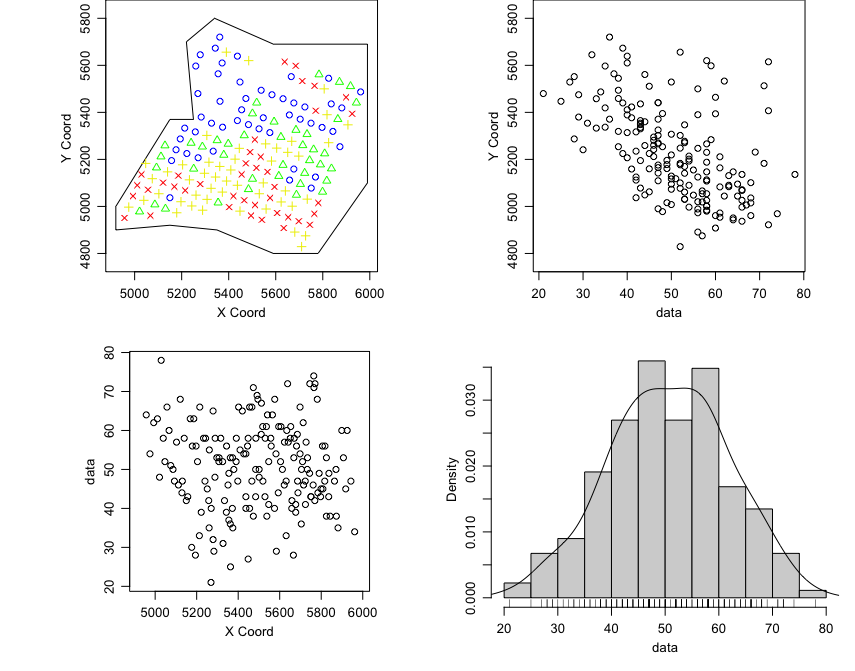
\includegraphics[width = \textwidth]{Rplot.png}
          \end{center}
        \end{figure}


        \item[b.] What is this data set? You can find documentation on it using the R command help(parana).\\
        \solution The data contains 178 observations of calcium content extracted from soil samples with 20cm depth. The area 
        of study was divided into 3 separate sub regions. Generally the data are calcium content, location (in long, lat pair) and elevation. The 
        area of each sub region was also recorded. Documentation from the help(ca20) function describes the data structures which store the data.
        \vspace{.15in}

        \item[c.] Describe the general features of this data set, e.g. N-S or E-W trend, if any; where are the values higher? Lower? WHat is the range of values in this 
        data set? Describe the shape of the distribution.\\
        \solution Looking at the first sub plot(top left) which shows the distribution of calcium samples across the sample region and recalling the hardcoded color values for the ordinal scale used to describe the data
        we see that there is a clear upward trend in the N-S direction. This is corroborated by the partial dependence subplot(top right) which shows a clear trend as the latitude decreases. The second partial dependence plot(bottom left)
        shows no clear trend with the longitude of the sample and it's calcium content. The final subplot(bottom right) shows that the values for calcium concentration from our sample look approximately normal, with good symmetry. We should note that our sample's distribution could 
        easily be bimodal if the sample region were two E-W transects separated by a substantial distance in the N-S direction. Beyond that unequal sampling on these transects would cause left or right skews. 
        \vspace{.15in}


        \item[d.] If the data needs to be log-transformed, include the 4-panel plot you get after transforming, and discuss the resulting plots; does it look as though this is an appropriate transformation.\\
        \solution The data does not appear to be skewed. I don't think log-transforming this data is necessary. 
        \vspace{.15in}

        \item[e.] Create ggplot versions of the four panel plots for the data on the original scale. Try changing some colors, font sizes, dot sizes.\\
        \solution\\
        \textbf{Code:}
        \begin{center}
        \lstinputlisting{r1.txt}
        \end{center}
        \begin{figure}[H]
          \begin{center}
          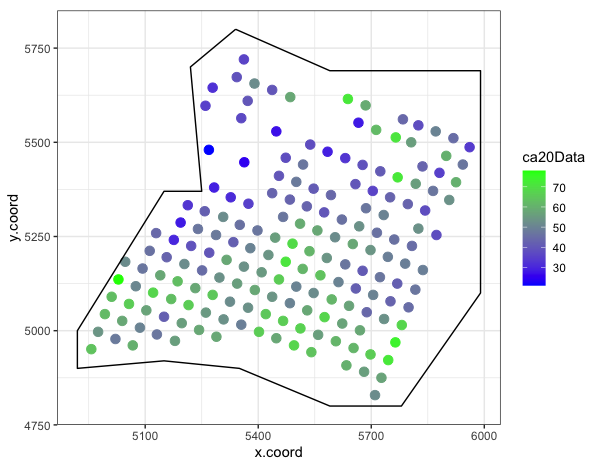
\includegraphics[width = .75\textwidth]{Rplot2.png}
          \end{center}
        \end{figure}
        \begin{figure}[H]
          \begin{center}
          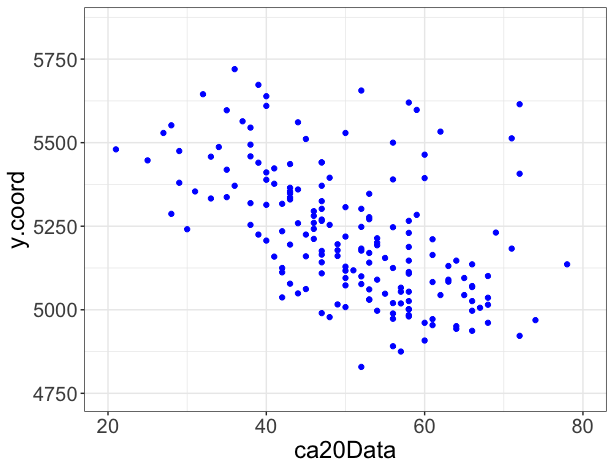
\includegraphics[width = .75\textwidth]{Rplot3.png}
          \end{center}
        \end{figure}
        \begin{figure}[H]
          \begin{center}
          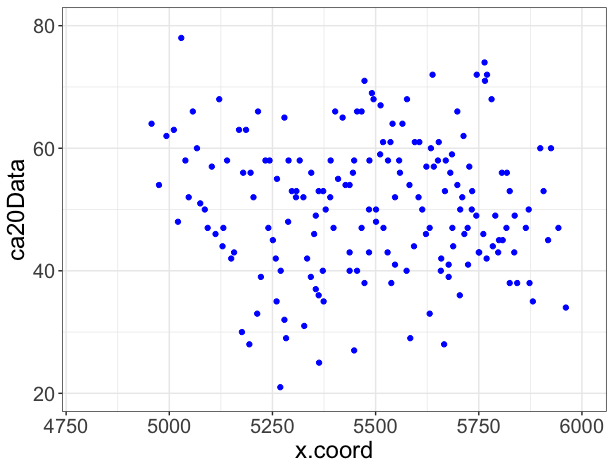
\includegraphics[width = .75\textwidth]{Rplot4.png}
          \end{center}
        \end{figure}
        \begin{figure}[H]
          \begin{center}
          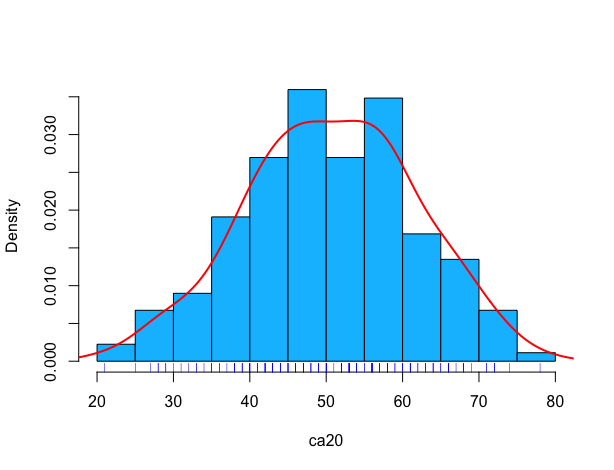
\includegraphics[width = .75\textwidth]{Rplot5.png}
          \end{center}
        \end{figure}
    \end{enumerate}
\end{exercise}
\vspace{1in}


\begin{exercise}{3} Repeats part (a)-(d) for the parana data set.\\
  \begin{enumerate}
    \item[a.] Plot the data set parana, using the plot function as illustrated on page 17 of the lecture notes.\\
    \solution  
    \begin{figure}[H]
      \begin{center}
      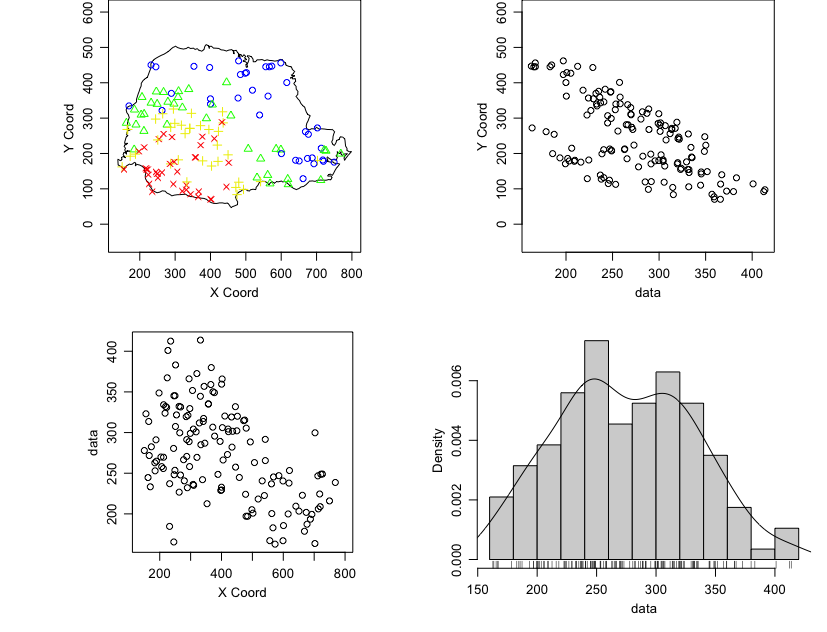
\includegraphics[width = \textwidth]{Rplot01.png}
      \end{center}
    \end{figure}
    \item[b.] What is this data set? You can find documentation on it using the R command help(parana).\\
    \solution This data set is average rainfall records at 143 different recording stations during the May-June spring season. 
    This information comes from the help(parana) command. 

    \item[c.]Describe the general features of this data set, e.g. N-S or E-W trend, if any; where are the values higher? Lower? What is the range of values in this 
        data set?\\ 
      \solution The first subplot shows us the distribution of weather stations, recalling the default color scale we know that the lowest values for average rainfall are 
      in the north east region. We can see that as we move from the north east to south west the average rainfall increases. This general trend is supported  by the partial dependce plots in the 
      second and third subplots (upper right and lower left respectively). The final subplot (lower right) shows the distribution of our data sample. We can see that it appears norma. and symmetric with a small
      dip near the mean, which might suggests we are looking at a bimodal sample. 

      \item[d.] If the data needs to be log-transformed, include the 4-panel plot you get after transforming, and discuss the resulting plots; does it look as though this is an appropriate transformation.\\
      \solution The data does not appear to be skewed. I don't think log-transforming this data is necessary. 
      \vspace{.15in}
  \end{enumerate}
\end{exercise}
\vspace{1in}


\begin{exercise}{4} Repeats part (a)-(d) for the wolfcamp data set.\\
  \begin{enumerate}
    \item[a.] Plot the data set wolfcamp, using the plot function as illustrated on page 17 of the lecture notes.\\
    \solution  
    \begin{figure}[H]
      \begin{center}
      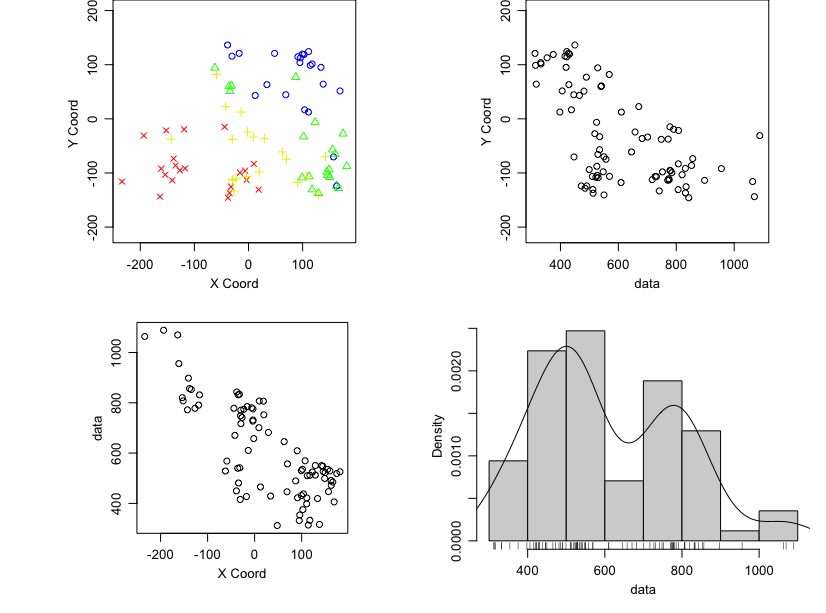
\includegraphics[width = \textwidth]{Rplot02.png}
      \end{center}
    \end{figure}
    \item[b.] What is this data set? You can find documentation on it using the R command help(wolfcamp).\\
    \solution This data set contains piezometric head measurements for the Wolfcamp aquifer in Texas. This is a measure of 
    pressure in an aquifer that is computed from the height of water in a tube. The data comes in long, lat pairs and head measurements. 



    \item[c.]Describe the general features of this data set, e.g. N-S or E-W trend, if any; where are the values higher? Lower? What is the range of values in this 
        data set?\\ 
      \solution The first subplot(top left) shows us the distribution of measurement stations for the Wolfcamp aquifer. It shows a clear trend of increasing pressure as we move 
      in the south west directions. The next two subplots show this trend in partial dependence plots. The final subplot(bottom right) shows a slight right skew in the distribution of 
      pressure measurements, along with possible bimodal-ness. 

      \item[d.] If the data needs to be log-transformed, include the 4-panel plot you get after transforming, and discuss the resulting plots; does it look as though this is an appropriate transformation.\\
      \solution The data does appear to be right skewed and looks like it could benefit from a log transform. Doing so we get the following plot, 
      \begin{figure}[H]
        \begin{center}
        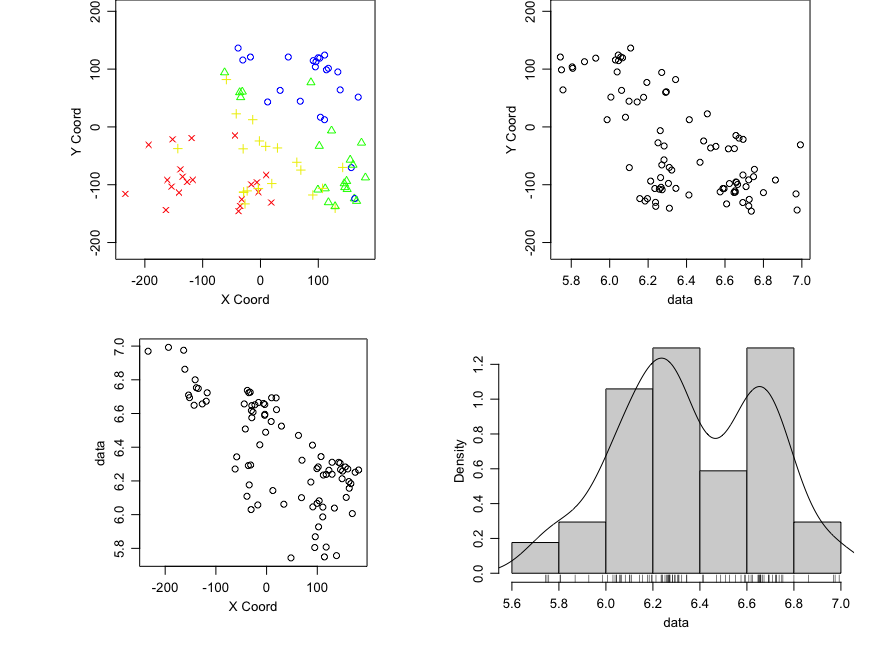
\includegraphics[width = \textwidth]{Rplot03.png}
        \end{center}
      \end{figure}
      The distribution of the data looks to be more centered and symmetric but is still exhibiting some bimodal-ness. 
  \end{enumerate}
\end{exercise}
\vspace{1in}





\begin{exercise}{5} We sometimes use the function $f(d) = exp(-d/\lambda)$ to express the correlation between observations 
  made at locations separated by the distance $d$, where $d \geq 0$. Here, $\lambda$ is a positive constant, which we treat as a known constant. \\
  \begin{enumerate}
    \item[a.] Show that $f(d) \geq 0$ and that $f(d) \leq 1$.\\
    \solution First note that the exponential function is continuous and differentiable across it's entire domain, that being the all real numbers. We also know 
    that function $f(x) = e^x$ in particular has a range from $(0, \infty)$. Let $x = -d/\lambda$ for some positive constant $\lambda$ and note that $f(d)$ has the same range 
    as $f(x)$, therefore it follows that there exist values of $d$ such that $f(d) > 0$ and $f(d) \leq 1$.
    \vspace{.15in}

    \item[b.] Let $\lambda = 1$. Find $d$ so that $f(d) = .05$.\\
    \solution Substituting $\lambda = 1$ to our function $f(d)$ we get, $f(d) = exp(-d)$. Solving for $d$, when $f(d) = .05$, 
    \begin{align*}
      .05 &= e^{-d}\\
      ln(.05) &= -d\\
      -ln(.05) &= d
    \end{align*}
    We get that the minimum distance between observations in order for them to be almost uncorrelated is $-ln(.05) \approx 3$. 
    \vspace{.15in}


    \item[c.] Let $\lambda = 5$. Find $d$ so that $f(d) = .05$\\
    \solution Substituting $\lambda = 5$ to our function $f(d)$ we get, $f(d) = exp(-d/5)$. Solving for $d$, when $f(d) = .05$, 
    \begin{align*}
      .05 &= e^{-d/5}\\
      5ln(.05) &= -d\\
      -5ln(.05) &= d
    \end{align*}
    We get that the minimum distance between observations in order for them to be almost uncorrelated is $-5ln(.05) \approx 15$. 
    \vspace{.15in}


    \item[d.] True/ False explain briefly. The larger $\lambda$ is, the quicker correlations die out with increased distance between observations. \\
    \solution False. Increasing $\lambda$ actually has the opposite effect on the slope of the function. Consider differentiating the function $f(d) = e^{d/\lambda}$. 
    We would get, $f'(d) = \frac{-1}{\lambda} e^{d/\lambda}$. The $\frac{-1}{\lambda}$ term shows us that the slope will decrease faster as $\lambda$ decreases. 
    \vspace{.15in}

    \item[e.] If $d$ is measured in km, what are the units for $\lambda$?.\\
    \solution Note that we are using $f(d)$ as a measure of correlation as a function of distance. Correlation is a unitless measure. Therefore we would want 
    $\lambda$ to be in the same units as $d$ to cancel them out.   
  \end{enumerate}
\end{exercise}
\vspace{1in}

\begin{exercise}{6} We sometimes use the function $f(d) = exp(-d\lambda)$ to express correlation between observations made at locations 
  separated by the distance $d$, $d \geq 0$. Here, $\lambda$ is a positive constant, which we treat as a known constant.\\
  \begin{enumerate}
    \item[a.] Let $\lambda = 5$. Find $d$ so that $f(d) = .05$. Compare this with your answer from 5c. \\
    \solution  Substituting $\lambda = 5$ and solving for $d$ we get, 
    \begin{align*}
      .05 &= e^{-d5},\\
      ln(.05) &= -d5,\\
      -\frac{ln(.05)}{5} &= d.
    \end{align*}
    Therefore we get a value for $d = -\frac{ln(.05)}{5} \approx .5$. This value is substantially less than the one given in 4c, which is as expected given 
    our explanation in 4c and our understanding of the derivative of the exponential function. \\
    \vspace{.15in}



    \item[b.] If $d$ is measured in km, what are the units for $\lambda$?\\
    \solution Similarly to 4e, we want to make our measure of correlation unitless. In order to do that for the function $f(d) = exp(-d\lambda)$
    $\lambda$ must have units in $1/km$. 
  \end{enumerate}
\end{exercise}
\vspace{1in}



\begin{exercise}{7} Logarithms using different bases.\\
  \begin{enumerate}
    \item[a.] Find $log_{10}(x)$ where $x = 2, 3, 4, 5$. Using R; - signif(log10(2:5), 4)\\
    \solution Using the stated R code we get the following values, 
    \begin{equation*}
      log_{10}(2) = .3010
    \end{equation*}
    \begin{equation*}
      log_{10}(3) = .4771
    \end{equation*} 
    \begin{equation*}
      log_{10}(4) = .6021
    \end{equation*} 
    \begin{equation*}
      log_{10}(5) = .6990
    \end{equation*} 
    \vspace{.15in}

    \item[b.] Find $ln(x)$ where $x = 2, 3, 4, 5$. Using R; - signif(log(2:5), 4).\\
    \solution Using the stated R code we get the following values, 
    \begin{equation*}
      ln(2) =  0.6931 
    \end{equation*}
    \begin{equation*}
      ln(3) = 1.0990 
    \end{equation*} 
    \begin{equation*}
      ln(4) = 1.3860 
    \end{equation*} 
    \begin{equation*}
      ln(5) = 1.6090
    \end{equation*} 
    \vspace{.15in}


    \item[c.] Find the ratios, $log_{10}/ln(x)$, where  $x = 2, 3, 4, 5$. Using R; -  signif(log10(2:5)/log(2:5), 4)\\
    \solution Using the stated R code we get the $log_{10}/ln(x) = .4343$ for all values of $x$. 
    \vspace{.15in}

    \item[d.] Find $log_{10}(e)$\\
    \solution Doing so in R we get, $log_{10}(e) = 0.4342945$. 
    \vspace{.15in}

    \item[e.] Find the ratios, $ln(x)/log_{10}$, where  $x = 2, 3, 4, 5$. Using R; -  signif(log(2:5)/log10(2:5), 4)\\
    \solution Using the stated R code we get the $ln(x)/log_{10} = 2.303$ for all values of $x$. 
    \vspace{.15in}

    \item[f.] Find ln(10)\\
    \solution Doing so in R we get, $ln(10) = 2.302585$
    \vspace{.15in}










  \end{enumerate}
\end{exercise}













\end{document}


















